% Title     :: SamzaSQL: Scalable Fast Data Management with Streaming SQL
% Author    :: Milinda Pathirage
% Email     :: mpathira@indiana.edu
% Website   :: http://milinda.pathirage.org
% Template  :: sthlm beamer theme by Benjamin Weiss (hendryolson@gmail.com, http://v42.com), 
%              which is HEAVILY based on the HSRM beamer theme created by Benjamin Weiss
%			   (benjamin.weiss@student.hs-rm.de), which can be found on GitHub
%			   <https://github.com/hsrmbeamertheme/hsrmbeamertheme>.



%-=-=-=-=-=-=-=-=-=-=-=-=-=-=-=-=-=-=-=-=-=-=-=-=
%
%        LOADING DOCUMENT
%
%-=-=-=-=-=-=-=-=-=-=-=-=-=-=-=-=-=-=-=-=-=-=-=-=

\documentclass[newPxFont]{beamer}
\usetheme{sthlm}
%\usecolortheme{sthlmv42}

%-=-=-=-=-=-=-=-=-=-=-=-=-=-=-=-=-=-=-=-=-=-=-=-=
%        LOADING PACKAGES
%-=-=-=-=-=-=-=-=-=-=-=-=-=-=-=-=-=-=-=-=-=-=-=-=
\usepackage[utf8]{inputenc}
\usepackage{hyperref}
\usepackage{minted}
\usepackage{xcolor}

\usepackage{chronology}

\renewcommand{\event}[3][e]{%
  \pgfmathsetlength\xstop{(#2-\theyearstart)*\unit}%
  \ifx #1e%
    \draw[fill=black,draw=none,opacity=0.5]%
      (\xstop, 0) circle (.2\unit)%
      node[opacity=1,rotate=45,right=.2\unit] {#3};%
  \else%
    \pgfmathsetlength\xstart{(#1-\theyearstart)*\unit}%
    \draw[fill=black,draw=none,opacity=0.5,rounded corners=.1\unit]%
      (\xstart,-.1\unit) rectangle%
      node[opacity=1,rotate=45,right=.2\unit] {#3} (\xstop,.1\unit);%
  \fi}%

%-=-=-=-=-=-=-=-=-=-=-=-=-=-=-=-=-=-=-=-=-=-=-=-=
%        BEAMER OPTIONS
%-=-=-=-=-=-=-=-=-=-=-=-=-=-=-=-=-=-=-=-=-=-=-=-=

%\setbeameroption{show notes}

%-=-=-=-=-=-=-=-=-=-=-=-=-=-=-=-=-=-=-=-=-=-=-=-=
%
%	PRESENTATION INFORMATION
%
%-=-=-=-=-=-=-=-=-=-=-=-=-=-=-=-=-=-=-=-=-=-=-=-=

\title{SamzaSQL}
\subtitle{Scalable Fast Data Management with \textit{Streaming SQL}}
%\date{\small{\jobname}}
%\date{\today}
\author{\textbf{Milinda Pathirage} (IU), Julian Hyde (Hortonworks), Yi Pan (LinkedIn), Beth Plale (IU)}
\institute{School of Informatics and Computing, Indiana University}

\hypersetup{
pdfauthor = {Milinda Pathirage: mpathira@indiana.edu},
pdfsubject = {},
pdfkeywords = {},
pdfmoddate= {D:\pdfdate},
pdfcreator = {}
}

\begin{document}
\setbeamertemplate{caption}{\raggedright\insertcaption\par}

%-=-=-=-=-=-=-=-=-=-=-=-=-=-=-=-=-=-=-=-=-=-=-=-=
%
%	TITLE PAGE
%
%-=-=-=-=-=-=-=-=-=-=-=-=-=-=-=-=-=-=-=-=-=-=-=-=

\maketitle

%\begin{frame}[plain]
%	\titlepage
%\end{frame}

%-=-=-=-=-=-=-=-=-=-=-=-=-=-=-=-=-=-=-=-=-=-=-=-=
%
%	TABLE OF CONTENTS: OVERVIEW
%
%-=-=-=-=-=-=-=-=-=-=-=-=-=-=-=-=-=-=-=-=-=-=-=-=

\section*{Introduction}

%-=-=-=-=-=-=-=-=-=-=-=-=-=-=-=-=-=-=-=-=-=-=-=-=
%	FRAME:
%-=-=-=-=-=-=-=-=-=-=-=-=-=-=-=-=-=-=-=-=-=-=-=-=

\begin{frame}[c]{Fast Data}

Data has to be process as it arrives, so that we can react to changing conditions fast. 

\vspace{1em}

\begin{exampleblock}{Big data isn't just big; it's also fast.}
Big data is often created by data that is generated at incredible speeds, such as click-stream data, financial ticker data, log aggregation, or sensor data. 
\end{exampleblock}
\vspace{-1.5em}
\begin{flushright}
\tiny\textit{John Hugg, \textbf{"Fast data: The next step after big data"}}
\end{flushright}

\end{frame}

%-=-=-=-=-=-=-=-=-=-=-=-=-=-=-=-=-=-=-=-=-=-=-=-=
%	FRAME:
%-=-=-=-=-=-=-=-=-=-=-=-=-=-=-=-=-=-=-=-=-=-=-=-=

\begin{frame}[c]{Lambda Architecture (LA)}
Technology agnostic data processing architecture that attempts to balance latency, accuracy, throughput and fault-tolerance by providing a unified serving layer on top of batch and stream processing sub-systems.   \\

\vspace{1em}

\begin{figure}
		\centering
		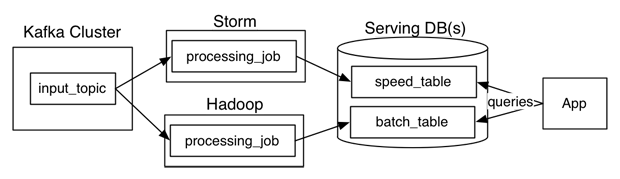
\includegraphics[width=0.75\linewidth]{lambda.png}
		\label{fig-lambda}
		\caption{\tiny\textit{From: \url{https://www.oreilly.com/ideas/questioning-the-lambda-architecture}}}
	\end{figure}

\end{frame}

%-=-=-=-=-=-=-=-=-=-=-=-=-=-=-=-=-=-=-=-=-=-=-=-=
%	FRAME:
%-=-=-=-=-=-=-=-=-=-=-=-=-=-=-=-=-=-=-=-=-=-=-=-=

\begin{frame}[c]{Kappa Architecture (KA)}
Simplification of \textit{Lambda Architecture} that uses append-only immutable log as the canonical data store and batch processing is replaced by stream replay. \\

\vspace{1em}

\begin{figure}
		\centering
		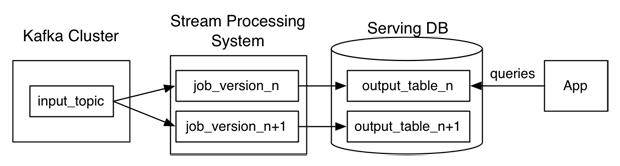
\includegraphics[width=0.75\linewidth]{kappa.png}
		\label{fig-lambda}
		\caption{\tiny\textit{From: \url{https://www.oreilly.com/ideas/questioning-the-lambda-architecture}}}
	\end{figure}

\end{frame}

%-=-=-=-=-=-=-=-=-=-=-=-=-=-=-=-=-=-=-=-=-=-=-=-=
%	FRAME:
%-=-=-=-=-=-=-=-=-=-=-=-=-=-=-=-=-=-=-=-=-=-=-=-=

%\begin{frame}[c]{sthlm Built on HSRM \& mTheme}
%\vspace{-1cm}
%\begin{center}\begin{chronology}[2]{2012}{2018}{0.85\textwidth}
%\event[\decimaldate{1}{1}{2013}]{\decimaldate{22}{9}{2013}}{hsrm theme}
%\event[\decimaldate{22}{9}{2013}]{\decimaldate{22}{8}{2014}}{sthlm based on hsrm}
%\event[\decimaldate{22}{8}{2014}]{\decimaldate{27}{4}{2015}}{branding sthlm for Stockholms stad}
%\event[\decimaldate{27}{4}{2015}]{\decimaldate{30}{8}{2015}}{\cRed{sthlm based on hsrm \& mTheme}}
%\end{chronology}
%\end{center}

%sthlm Theme is heavily based on the work of Benjamin Weiss \alert{HSRM} and Matthias Vogelgesang \alert{mTheme}.

%\end{frame}

%\section*{Overview}
%\begin{frame}{Overview}
% For longer presentations use hideallsubsections option
%\tableofcontents[hideallsubsections]
%\end{frame}


%-=-=-=-=-=-=-=-=-=-=-=-=-=-=-=-=-=-=-=-=-=-=-=-=
%
%	SECTION: Motivation
%
%-=-=-=-=-=-=-=-=-=-=-=-=-=-=-=-=-=-=-=-=-=-=-=-=

\section*{Motivation}

%-=-=-=-=-=-=-=-=-=-=-=-=-=-=-=-=-=-=-=-=-=-=-=-=
%	FRAME:
%-=-=-=-=-=-=-=-=-=-=-=-=-=-=-=-=-=-=-=-=-=-=-=-=

\begin{frame}{SQL for Big Data}

There are sevaral well known SQL-on-Hadoop solutions and most organisations that use Hadoop use one or more SQL-on-Hadoop solutions.

\begin{itemize}
	\item Apache Hive
	\item Presto
	\item Apache Drill
	\item Apache Impala
	\item Apache Kylin
	\item Apache Tajo
	\item Apache Pheonix
\end{itemize}

\end{frame}

%-=-=-=-=-=-=-=-=-=-=-=-=-=-=-=-=-=-=-=-=-=-=-=-=
%	FRAME: 
%-=-=-=-=-=-=-=-=-=-=-=-=-=-=-=-=-=-=-=-=-=-=-=-=

\begin{frame}{Programming APIs for LA and KA}

\href{https://github.com/twitter/summingbird}{\textbf{Summingbird}} is a well known abstraction for writing \textit{LA} style applications while \textit{KA} style applications were mainly written in \textbf{stateful stream processing APIs} provided by frameworks like \href{http://samza.apache.org}{Apache Samza}.

\begin{block}{Limitations}
\begin{itemize}
	\item Need to maintain two complex distributed systems
	\item Users need to understand various programming abstractions 
	\item Long turnaround times
\end{itemize}
\end{block}

\end{frame}

%-=-=-=-=-=-=-=-=-=-=-=-=-=-=-=-=-=-=-=-=-=-=-=-=
%	FRAME: 
%-=-=-=-=-=-=-=-=-=-=-=-=-=-=-=-=-=-=-=-=-=-=-=-=

\begin{frame}[fragile]{Summingbird}
\begin{exampleblock}{Word Count}
\begin{minted}[
framesep=2mm,
baselinestretch=1.2,
fontsize=\footnotesize,
]{scala}
def wordCount[P <: Platform[P]]
    (source: Producer[P, String], store: P#Store[String, Long]) =
      source.flatMap { sentence =>
        toWords(sentence).map(_ -> 1L)
      }.sumByKey(store)
\end{minted}
\end{exampleblock}
\vspace{-1.5em}
\begin{flushright}
\tiny\textit{More examples at \url{https://github.com/twitter/summingbird}}
\end{flushright}
\end{frame}

%-=-=-=-=-=-=-=-=-=-=-=-=-=-=-=-=-=-=-=-=-=-=-=-=
%	FRAME: 
%-=-=-=-=-=-=-=-=-=-=-=-=-=-=-=-=-=-=-=-=-=-=-=-=

\begin{frame}[fragile]{Samza API}
\begin{exampleblock}{Window Aggregation}
\begin{minted}[
framesep=0mm,
%baselinestretch=1.2,
fontsize=\tiny,
]{java}
public class WikipediaStatsStreamTask implements StreamTask, InitableTask, WindowableTask {
  ...
  private KeyValueStore<String, Integer> store;
  public void init(Config config, TaskContext context) {
    this.store = (KeyValueStore<String, Integer>) context.getStore("wikipedia-stats");
  }
  @Override
  public void process(IncomingMessageEnvelope envelope, MessageCollector collector, 
                      TaskCoordinator coordinator) {
    Map<String, Object> edit = (Map<String, Object>) envelope.getMessage();
    ...
  }
  @Override
  public void window(MessageCollector collector, TaskCoordinator coordinator) {
    ...
    collector.send(new OutgoingMessageEnvelope(new SystemStream("kafka", "wikipedia-stats"), counts));
    ...
  }
\end{minted}
\end{exampleblock}

\end{frame}

%-=-=-=-=-=-=-=-=-=-=-=-=-=-=-=-=-=-=-=-=-=-=-=-=
%	FRAME: 
%-=-=-=-=-=-=-=-=-=-=-=-=-=-=-=-=-=-=-=-=-=-=-=-=

\begin{frame}{Motivating Research Question}
\Large{Can the same low barrier and the clear semantics of SQL be extended to queries that execute simultaneously over data \texttt{\textbf{streams}} (in movement) and \texttt{\textbf{tables}} (at rest)?} \\

\Large{Can this be done with minimal and well-founded extensions to SQL?}
\end{frame}
%-=-=-=-=-=-=-=-=-=-=-=-=-=-=-=-=-=-=-=-=-=-=-=-=
%
%	SECTION: UPDATESS
%
%-=-=-=-=-=-=-=-=-=-=-=-=-=-=-=-=-=-=-=-=-=-=-=-=

\section{SamzaSQL}

%-=-=-=-=-=-=-=-=-=-=-=-=-=-=-=-=-=-=-=-=-=-=-=-=
%	FRAME:
%-=-=-=-=-=-=-=-=-=-=-=-=-=-=-=-=-=-=-=-=-=-=-=-=

\begin{frame}[c]{Streaming SQL}

\end{frame}




%-=-=-=-=-=-=-=-=-=-=-=-=-=-=-=-=-=-=-=-=-=-=-=-=
%
%	SECTION: Conclusion
%
%-=-=-=-=-=-=-=-=-=-=-=-=-=-=-=-=-=-=-=-=-=-=-=-=

\begin{frame}{Conclusion}

\end{frame}

\end{document}